\providecommand{\main}{..}
\documentclass[\main/master.tex]{subfiles}
\begin{document}
\chapter{methods and results}\label{chp:example-2}
\section{vacuum system}







\section{torsion pendulum system}
The angle of torsion is measured using a mirror connected in front of the pendulum.This mirror is a part of an optical interferometer with which the mirror tilt could bedetermined.In order to balance the pendulum so the mirror would not be tilted, beside the tiltof the gravity field. The center of mass needs to be adjusted. The center of mass isadjusted using a mass from the back, to balance the mirror weight.The longer the wire and the smaller the wire diameter - wire torsion coefficient issmaller. Small coefficient achieves a better angle response to the gravity field. On theother hand the Small coefficient is leading to a very long time period of the pendulum,which while integrating over time would lead to very long measurements time. Alsothe wire needs to be strong enough to hold the masses without been teared down.


\section{Modulated CW Laser}

\subsection{Laser}


The laser is a high power coherent light source based on stimulated emmission with narrow spectrum. Inside a cavity Electron is excited to a higher energy level, and forced by photon with the correct wavelength to be absorbed emmiting coherent photon. The coherence allows focusing beam to a tight spot, and being collimated over long distances. Continuous wave (CW) laser are lasing constant output power over time.



\par
Usually the power output is stable but has oscillations due to having several longitudinal modes causing nano second scale ossicilations, output power is steady when averaged over longer periods. Also, over long periods of time lasers have slight power oscillations due to temperture changes in the envirement.
%The laser diode cavity face is rectangular, because of fabrication constraints. The rectangular face is causing cylindrical aberration, which   

\subsection{Acousto Optic Modulator}
Acousto Optic Modulator (AOM), uses the acousto-optic effect to diffract and shift the frequency of light using RF waves. An oscillating electric signal drives a piezoelectric transducer to vibrate causing RF waves, the transducer attached to a material. This causes sound waves in the material, and periodic index modulation causing a Bragg grating. Incoming light scatters off the grating and due to Bragg diffraction comes at Bragg angle.
\begin{equation}
\theta_b = sin(\theta_b)\approx \frac{\lambda}{2n\Lambda} \label{eqn:energy-mass-equivalence-relation}
\end{equation} 
$\Lambda$ is the RF wavelength, $\lambda$ is the light source wavelength. 
\par
Since all parameters constant, modulation angle is constant, and possible modulation speed is nano seconds. Giving a stable fast modulation method for CW laser.


\section{Modulated LED}
\subsection{arduino}
Arduino is an open-source microcontroller board used for building low cost and simple digital devices and circuits. Each microcontroller contains a microprocessor, controller, serial communication interface and is equipped with digital and analog input/output pins. The microcontrollers could be operated as stand alone or connected to computer through serial communication. 
\par
The Arduino Mega 2560, based on the ATmega2560 8-bit controller, is equiped with 16 MHz crystal oscillator (clock) and 15 PWM outputs pins. Arduino doesn't have analog output, but is simulates analog output using Pulse Width Modulation.
\par
The controller switches the output signal between the board Vcc (which is a digital 5[V]) and off, generating a square wave.
Repeating the pattern fast enough results in an analog signal as if the signal is a steady voltage. The time signal duration called the pulse width. Controller is modulating with clock the pulse width, changing the ratio time signal is on compare to off. 
\par
Output voltage is determined by that ratio, which is called duty cycle. 100\% duty cycle meaning power is always on and output is the full Vcc, 0\% power off and 50\% signal is on and off equally resulting with output of half. 
\par
The method enables generating signals between board Vcc and off. Signal resolution limited by the microcontroller resolution (8-bit). Due to the fast arduino clock possible signal modulation frequency is up to 500Hz.
\par
Since clock is connected to all PWM pins, they are in sync. When all pins have the same duty cycle, they all have the same voltage over time. At every point in time they could be looked at as a constant voltage supplies compare to each other, alowing to connect them in series and increase the output current up to 1[A]. 
\subsection{Light Emitting Diode (LED)}
The light emitting diode (led) is a high power long lifetime light source semiconductor based. The led is emitting light when current flows through. Led could be modulated at up to 100MHz. The initial opening angle of a led source varies between 45 to 120 degrees. The emitted light is incoherent in width meaning it's hard to focus it to a point (not diffraction limited). The emitted light is incoherent in length causing wide band spectrum.
\par
\par
Forward voltage is applied causing electron injection and recombination with holes. The recombination is releasing energy in form of spontanious emmission photons. The modulation limitation is due to the electrons life time before recombination. The led power is proptional to the current flows through, Shockley diode equation for p-n junction defines the current relation to the diode voltage. In high enough values the power could be aproximated by liniar aproximation of the diode voltage.
\begin{equation}
P\propto e^{\frac{q}{kT}\cdot V_d}\label{eqn:energy-mass-equivalence-relation}
\end{equation}
In order to overcome the led uncoherent profile and large opening angle, light was transfered through a light guide. Light guides are pipes made of thin filaments causing internal reflections used for directed transmission of luminous energy. Light guides are used to illuminate small areas, regardless of the spectral characteristics of the light source. They mainly depend on the cross sections of entrance and exit and the length. Making them ideal to overcoming focusing problems.
\par
Connecting a high power led to arduino, enables fast real-time controlled modulation of high power led with about 2ms speed. The light arrives to pendulum through a light guide allowing to assume beam variation through the surface neglegible.The light is controlled through a PID and applies a tourqe.
\par
Since the led power could be aproximated using liniar aproximation, the power modulation is propotional to the arduino duty cycle. That allows to control the liniar aproximation of the power output by changing the PID gain values.  
\par
we assume we can neglect the ossiclations between two sides...



\begin{figure}[htbp]
	\centering
	\fbox{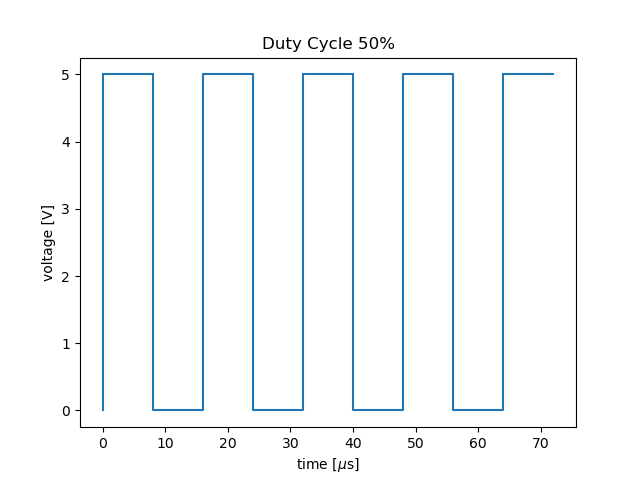
\includegraphics[scale=0.5]{\main/images/devices/duty50.png}}
	\caption[duty cycle 50\%]{50\% duty cycle  - signal is on and off equal times}
	\label{fig:duty50}
\end{figure}
 
\begin{figure}[htbp]
	\centering
	\fbox{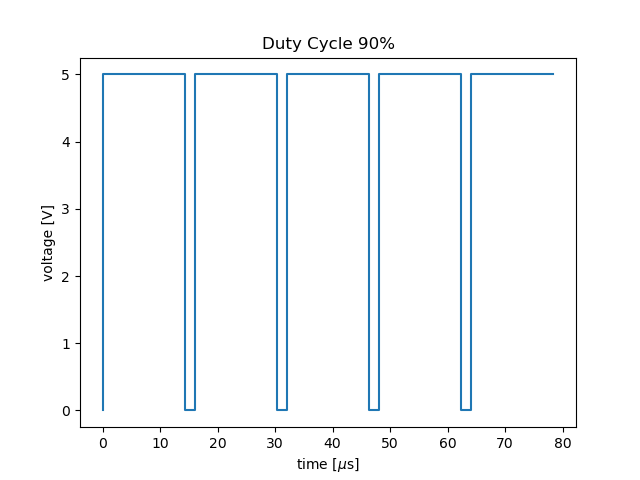
\includegraphics[scale=0.5]{\main/images/devices/duty90.png}}
	\caption[duty cycle 90\%]{90\% of the time signal on, equivalamt to 90\% of the full Vcc signal}
	\label{fig:duty90}
\end{figure}














\section{pid operate (algoritm)}
\section{laser +aom}
\section{laser +aom +amp}
\section{arduino + led}
\doublespacing
\hspace{5 mm} This another example chapter with a working reference as see in Chapter~\ref{chp:example-1}. There I also made an example of an equation, see Eqn.~\ref{eqn:energy-mass-equivalence-relation}. We also created an example image, see Fig.~\ref{fig:sine-wave}.
\begin{figure}[htbp]
	\centering
	\fbox{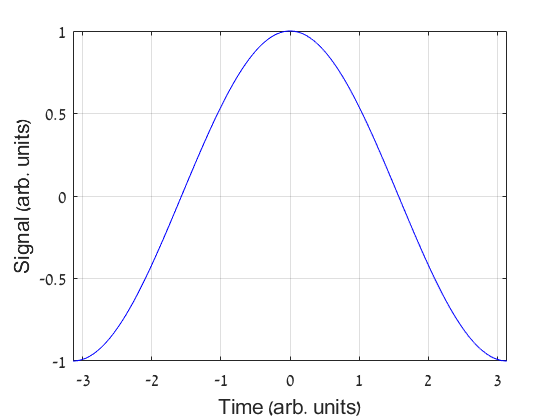
\includegraphics[scale=0.75]{\main/images/chapter_2_example/img_example_2.png}}
	\caption[Another Example Image]{Another Example Image. This image is also labeled internally so we can referenc it throughout the text.}
	\label{fig:cosine-wave}
\end{figure}


\section{Overshoot}
Overshoot is when output signal or function exceeds the target value. The response signal is not accurate compare to target. In controll theory there are two wanted conflicting properties; an accurate response (small overshoot), and small risetime (fast response). 
\par
Overshoot is usually measured in percentage overshoot (PO). For second order systems, such as damped oscillators PO is a function of the damping ratio $\xi$. 


\begin{equation}
PO = 100\cdot e ^{\frac{-\xi\pi}{\sqrt{1-\xi^2}}} = \frac{output-target}{target}   \label{eqn:percentage_overshoot}
\end{equation}
 

\end{document}